\documentclass[a4paper,14pt]{extarticle}

\usepackage{tikz,amsmath,graphicx,xcolor}
\usepackage[a4paper,landscape,margin=-2mm]{geometry}

\usepackage[utf8x]{inputenc}
\usepackage[T2A]{fontenc}
\usepackage[russian]{babel}

\begin{document}
\pagestyle{empty}

\def\hAt{-2}

\definecolor{cm}{RGB}{190,0,170}
\definecolor{half}{RGB}{45,190,80}
\definecolor{each}{RGB}{215,215,215}

\def\vertgrid{
	\foreach \y in {-6,...,4} {
		\draw[color=cm,very thick] (\hAt cm - 0.8 cm,\y cm)
			node[left]{\y}
			-- (\hAt cm - 0.4 cm,\y cm);
		\foreach \t in {1,...,9} {
			\draw[color=each,thick] (\hAt cm - 0.68 cm, \y cm + 0.1*\t cm)
				-- (\hAt cm - 0.52 cm, \y cm + 0.1*\t cm);
		};
		\draw[color=half,very thick]
			(\hAt cm - 0.71 cm, \y cm + 0.5 cm)
			-- (\hAt cm - 0.49 cm, \y cm + 0.5 cm);
	};
}

\begin{center} \tikz{
	\draw (0,0) node{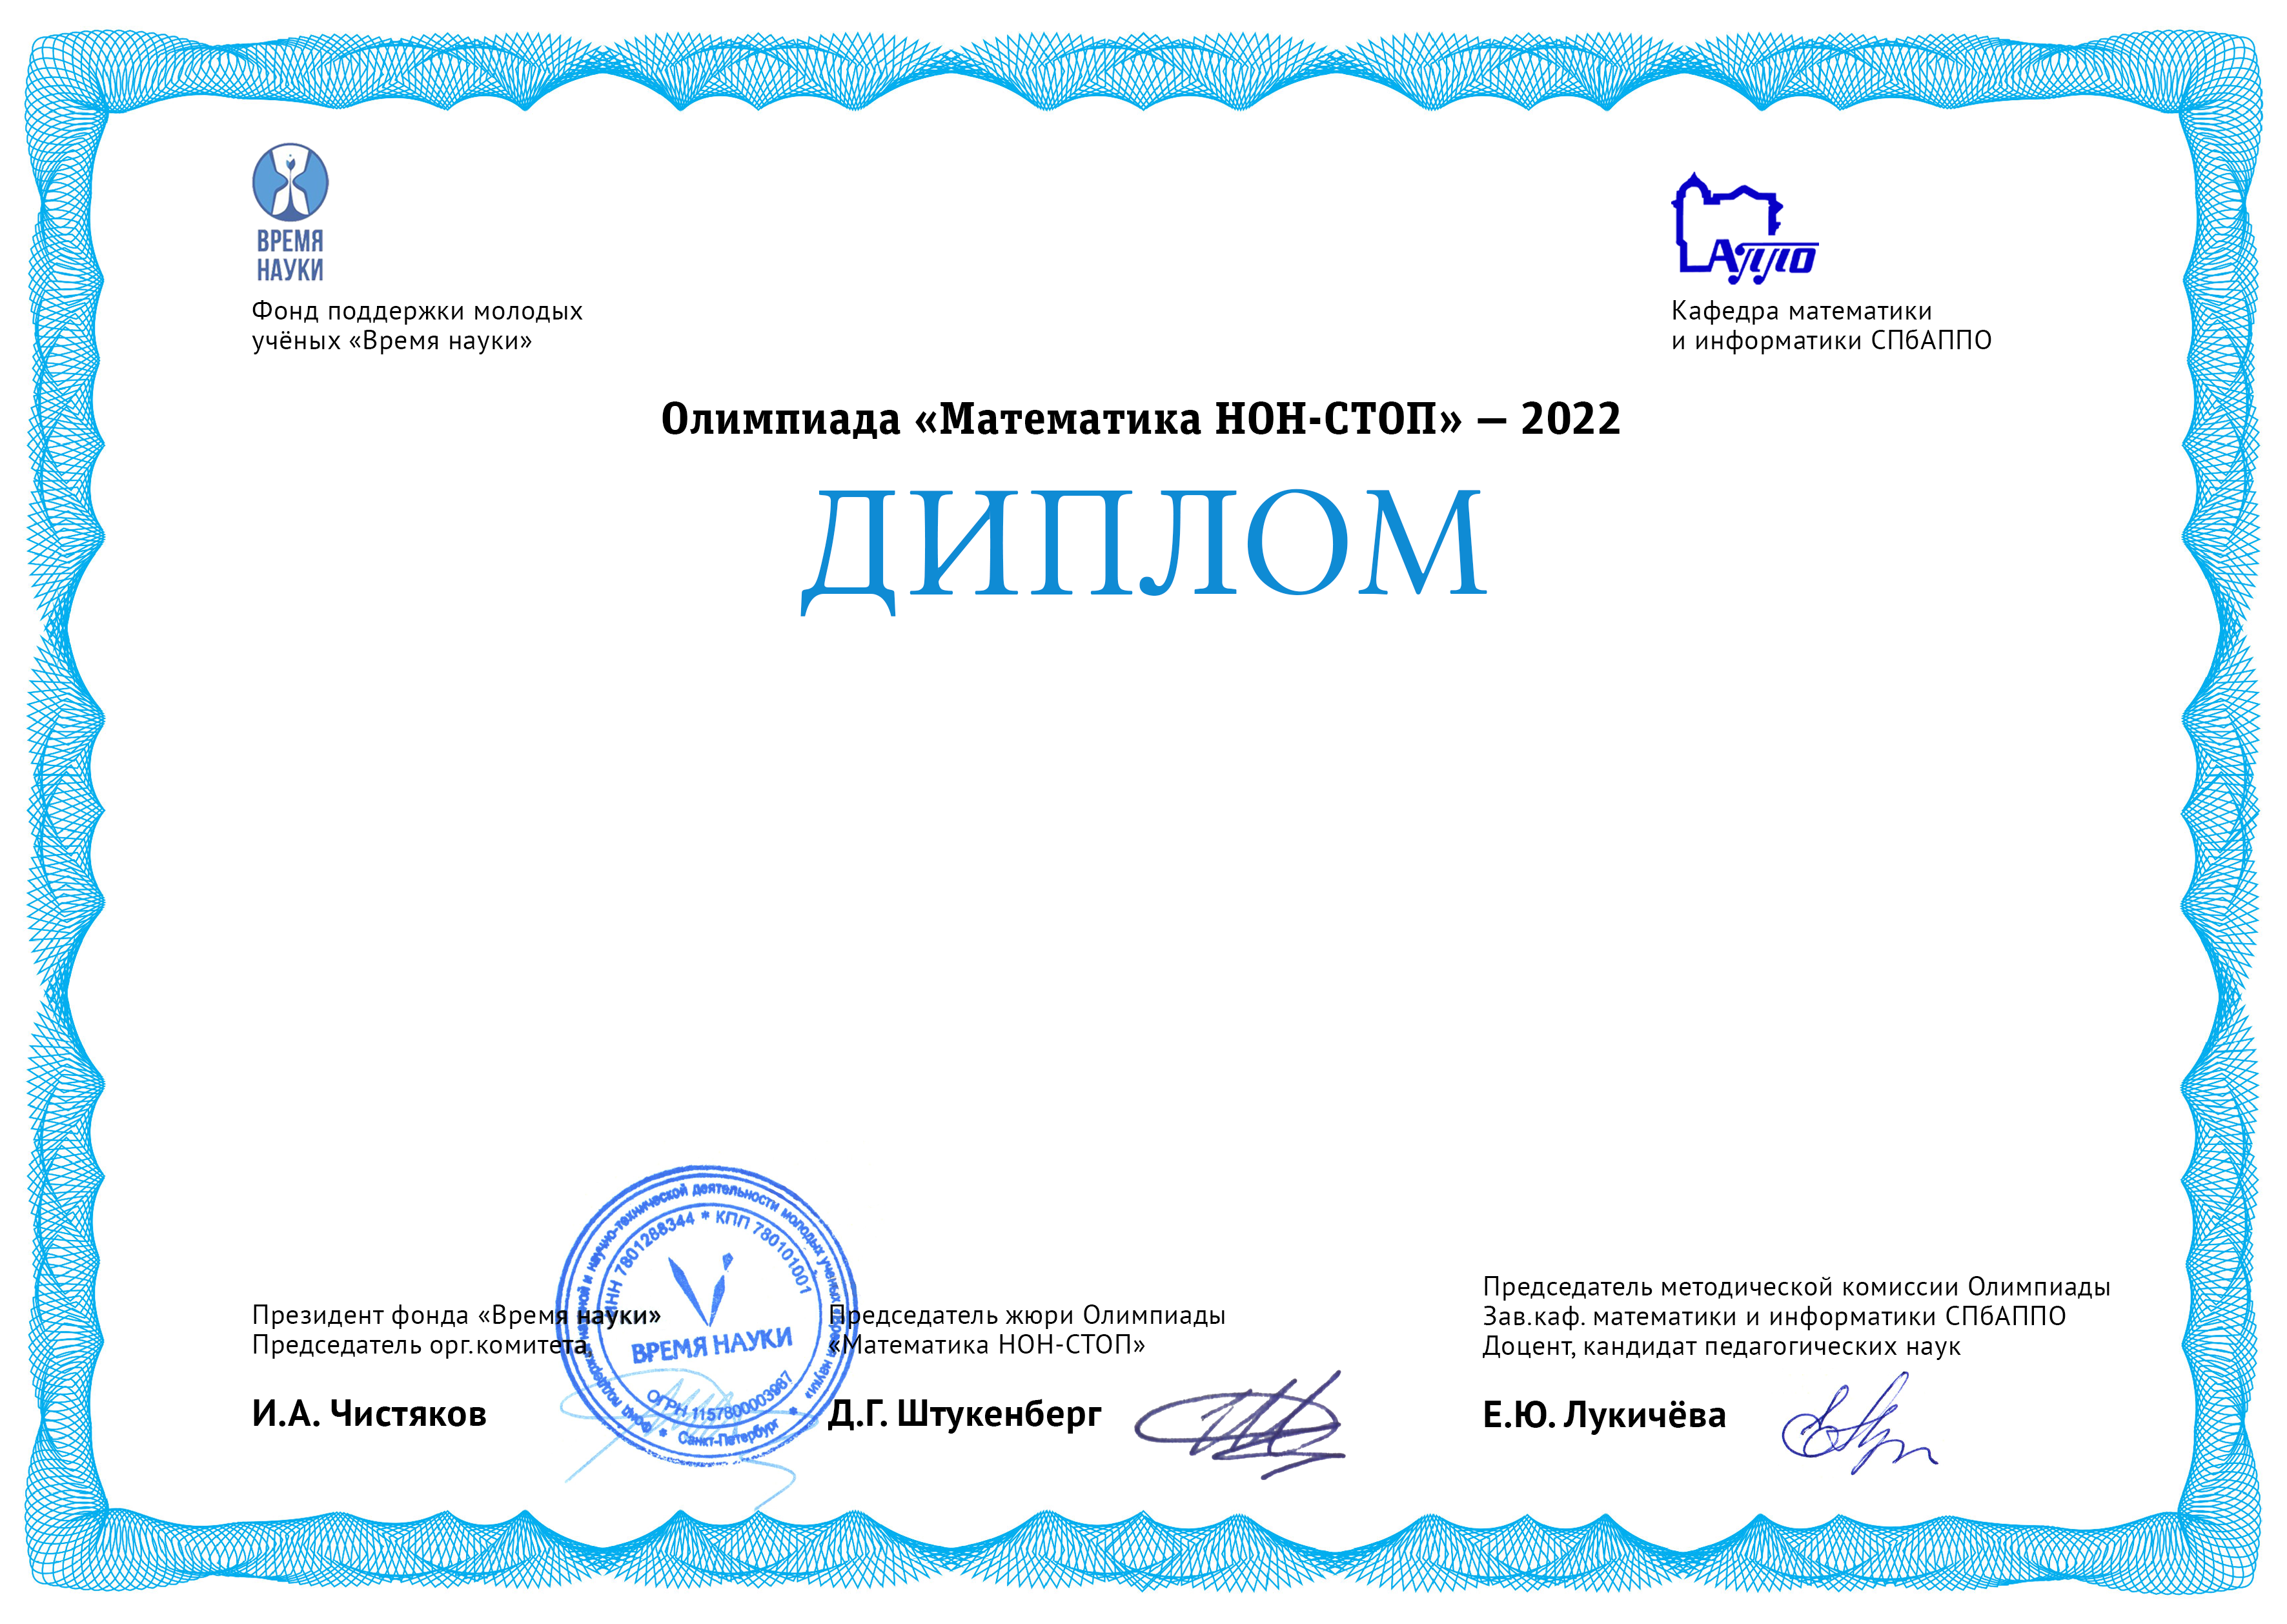
\includegraphics[width=29cm]{2022t}};
	\draw (0,1.5) node{\LARGE\bfseries второй степени};
	\draw (0,-0.2) node{\huge\bfseries Пахолкова Алиса Александровна};
	\draw (0,-1.6) node{\Large\itshape ГБОУ СОШ №630 Приморского района};
	\draw (0,-2.75) node{\Large\itshape 4 класс, вариант 4-базовый};
%	\vertgrid;
} \end{center}

\end{document}
